\documentclass[tikz,border=4pt]{standalone}
\usepackage[T1]{fontenc}
\usepackage{lmodern}
\usepackage{amsmath}
% Shared TikZ style for the report figures.
% Colours follow the Okabe-Ito palette, which stays distinguishable under the
% common forms of colour-vision deficiency. Every colour-coded element also
% carries a text label, so no figure depends on colour alone.
\usetikzlibrary{arrows.meta,positioning,fit,calc,backgrounds,decorations.pathreplacing,shapes.geometric}

\definecolor{oiOrange}{HTML}{E69F00}
\definecolor{oiSky}{HTML}{56B4E9}
\definecolor{oiGreen}{HTML}{009E73}
\definecolor{oiYellow}{HTML}{F0E442}
\definecolor{oiBlue}{HTML}{0072B2}
\definecolor{oiVerm}{HTML}{D55E00}
\definecolor{oiPurple}{HTML}{CC79A7}
\definecolor{oiGray}{HTML}{6E6E6E}

\colorlet{corTreino}{oiBlue!22}
\colorlet{corValid}{oiGreen!30}
\colorlet{corTeste}{oiOrange!45}
\colorlet{corControle}{oiPurple!35}

\tikzset{
  >=Stealth,
  bloco/.style={draw=black!70, rounded corners=1.5pt, minimum height=0.62cm,
    inner sep=2pt, font=\sffamily\fsz, align=center},
  treino/.style={bloco, fill=corTreino},
  valid/.style={bloco, fill=corValid},
  teste/.style={bloco, fill=corTeste, thick},
  etapa/.style={draw=black!70, rounded corners=3pt, fill=black!4,
    text width=4.3cm, align=center, inner sep=4pt, font=\sffamily\fsz},
  nota/.style={font=\sffamily\fsz, align=left, text=black!80},
  titulo/.style={font=\sffamily\fst\bfseries, anchor=west},
  seta/.style={->, thick, black!70},
  regiao/.style={draw=black!50, dashed, rounded corners=4pt},
}

% Absolute font sizes, so a figure looks the same standalone (10 pt class) and
% inside the 11 pt report.
\providecommand{\fsx}{\fontsize{5.5}{6.5}\selectfont}
\providecommand{\fsz}{\fontsize{7}{8.5}\selectfont}
\providecommand{\fst}{\fontsize{9}{11}\selectfont}

\begin{document}
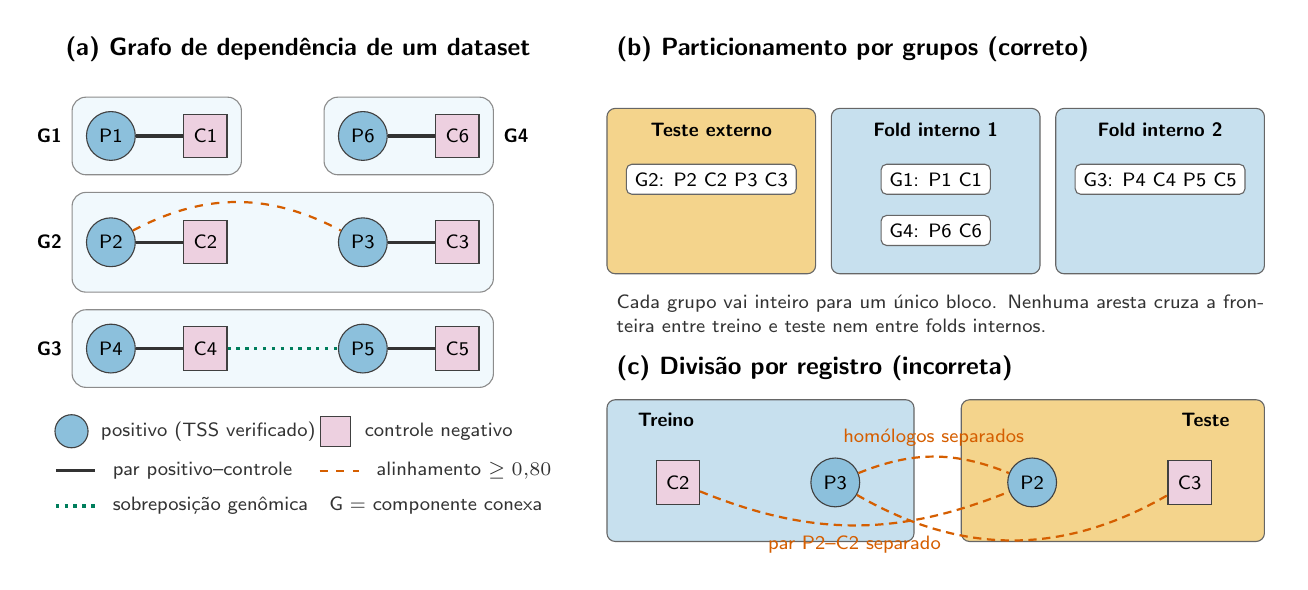
\begin{tikzpicture}[
  posit/.style={circle, draw=black!75, fill=oiBlue!45, minimum size=0.62cm, inner sep=0pt, font=\sffamily\fsz},
  ctl/.style={rectangle, draw=black!75, fill=corControle, minimum size=0.55cm, inner sep=0pt, font=\sffamily\fsz},
  par/.style={very thick, black!80},
  homol/.style={thick, dashed, oiVerm},
  sobrep/.style={very thick, dotted, oiGreen!80!black},
  grupo/.style={draw=black!45, rounded corners=5pt, inner sep=5pt},
  chip/.style={draw=black!60, rounded corners=2pt, fill=white, font=\sffamily\fsz, inner sep=3pt},
  vaz/.style={thick, oiVerm, densely dashed},
  ]
  % ---------------- (a) dependency graph ----------------
  \node[titulo] at (0,0.2) {(a) Grafo de dependência de um dataset};
  \node[posit] (P1) at (0.7,-0.9) {P1}; \node[ctl] (C1) at (1.9,-0.9) {C1};
  \node[posit] (P6) at (3.9,-0.9) {P6}; \node[ctl] (C6) at (5.1,-0.9) {C6};
  \node[posit] (P2) at (0.7,-2.25) {P2}; \node[ctl] (C2) at (1.9,-2.25) {C2};
  \node[posit] (P3) at (3.9,-2.25) {P3}; \node[ctl] (C3) at (5.1,-2.25) {C3};
  \node[posit] (P4) at (0.7,-3.6) {P4}; \node[ctl] (C4) at (1.9,-3.6) {C4};
  \node[posit] (P5) at (3.9,-3.6) {P5}; \node[ctl] (C5) at (5.1,-3.6) {C5};
  \foreach \i in {1,...,6} { \draw[par] (P\i) -- (C\i); }
  \draw[homol] (P2) to[bend left=28] (P3);
  \draw[sobrep] (C4) -- (P5);
  \begin{scope}[on background layer]
    \node[grupo, fill=oiSky!8, fit=(P1)(C1), label={[font=\sffamily\fsz\bfseries]left:G1}] {};
    \node[grupo, fill=oiSky!8, fit=(P6)(C6), label={[font=\sffamily\fsz\bfseries]right:G4}] {};
    \node[grupo, fill=oiSky!8, fit=(P2)(C3)(C2)(P3), inner ysep=9pt, label={[font=\sffamily\fsz\bfseries]left:G2}] {};
    \node[grupo, fill=oiSky!8, fit=(P4)(C5), label={[font=\sffamily\fsz\bfseries]left:G3}] {};
  \end{scope}
  % legend
  \begin{scope}[shift={(0,-4.65)}]
    \node[posit, minimum size=0.42cm] at (0.2,0) {}; \node[nota, anchor=west] at (0.45,0) {positivo (TSS verificado)};
    \node[ctl, minimum size=0.38cm] at (3.55,0) {}; \node[nota, anchor=west] at (3.8,0) {controle negativo};
    \draw[par] (0,-0.5) -- (0.5,-0.5); \node[nota, anchor=west] at (0.6,-0.5) {par positivo--controle};
    \draw[homol] (3.35,-0.5) -- (3.85,-0.5); \node[nota, anchor=west] at (3.95,-0.5) {alinhamento $\geq 0{,}80$};
    \draw[sobrep] (0,-0.95) -- (0.5,-0.95); \node[nota, anchor=west] at (0.6,-0.95) {sobreposição genômica};
    \node[nota, anchor=west] at (3.35,-0.95) {G = componente conexa};
  \end{scope}

  % ---------------- (b) group-safe partition ----------------
  \node[titulo] at (7.0,0.2) {(b) Particionamento por grupos (correto)};
  \foreach \nome/\x/\cor in {Teste externo/7.0/corTeste, Fold interno 1/9.85/corTreino, Fold interno 2/12.7/corTreino} {
    \draw[draw=black!60, fill=\cor, rounded corners=3pt] (\x,-0.55) rectangle ++(2.65,-2.1);
    \node[font=\sffamily\fsz\bfseries] at (\x+1.325,-0.82) {\nome};
  }
  \node[chip] at (8.325,-1.45) {G2: P2 C2 P3 C3};
  \node[chip] at (11.175,-1.45) {G1: P1 C1};
  \node[chip] at (11.175,-2.1) {G4: P6 C6};
  \node[chip] at (14.025,-1.45) {G3: P4 C4 P5 C5};
  \node[nota, anchor=north west, text width=8.3cm] at (7.0,-2.8)
    {Cada grupo vai inteiro para um único bloco. Nenhuma aresta cruza a fronteira entre treino e teste nem entre folds internos.};

  % ---------------- (c) record-level split ----------------
  \node[titulo] at (7.0,-3.85) {(c) Divisão por registro (incorreta)};
  \draw[draw=black!60, fill=corTreino, rounded corners=3pt] (7.0,-4.25) rectangle (10.9,-6.05);
  \draw[draw=black!60, fill=corTeste,  rounded corners=3pt] (11.5,-4.25) rectangle (15.35,-6.05);
  \node[font=\sffamily\fsz\bfseries] at (7.75,-4.5) {Treino};
  \node[font=\sffamily\fsz\bfseries] at (14.6,-4.5) {Teste};
  \node[ctl] (xC2) at (7.9,-5.3) {C2};  \node[posit] (xP3) at (9.9,-5.3) {P3};
  \node[posit] (xP2) at (12.4,-5.3) {P2}; \node[ctl] (xC3) at (14.4,-5.3) {C3};
  \draw[vaz] (xC2) to[bend right=22] node[below, nota, text=oiVerm, pos=0.5] {par P2--C2 separado} (xP2);
  \draw[vaz] (xP3) to[bend left=22] node[above, nota, text=oiVerm, pos=0.5] {homólogos separados} (xP2);
  \draw[vaz] (xP3) to[bend right=30] (xC3);
\end{tikzpicture}
\end{document}
